\section{Introduction}
\label{sec:introduction}
% \begin{itemize}
%     \item Mechanical computing uses deformation and mechanical motion for data storage and computation.
%     \item Applicable in intelligent mechanical systems like soft devices, MEMS, and robotic materials.
%     \item Limitation: Inefficient data exchange between memory and computing modules hampers performance.
%     \item Logic gates realized through origami, buckled beams, and mechanical linkages.
%     \item Signal propagation via mechanical, mechano-electronic, and mechanical-fluidic interfaces.
%     \item Non-volatile mechanical memory exists but requires complex peripherals or intricate energy landscapes.
%     \item Consideration: Cellular automata as a potential architecture to address data exchange bottleneck.
% \end{itemize}


% xMaterials that couple sensing, actuation, computation, and communication \cite{McEvoy2015}
% Mechanical Computation, Redux? \cite{ Roukes2004}
% Programmable Mechanical Metamaterials \cite{Florijn2014}
% Programmable matter: Concepts and realization \cite{Margolus1996}
% Functional mechanical metamaterials - development of programmable mechanical structures \cite{Waheed2022}
% Mechanical Computing Systems Using Only Links and Rotary Joints \cite{Merkle2018}
% A mechanical metamaterial with reprogrammable logical functions \cite{ Mei2021}
% Mechanical reversible logic without sliding contacts \cite{ Merkle1993}
% Mechanical metamaterials can count and process sequential information \cite{Kwakernaak2022}
% A New Kind of Science \cite{ Wolfram2002}
% Computation in Cellular Automata: A Selected Review \cite{ Mitchell1996}
% Universality in Elementary Cellular Automata \cite{ Cook1985}
% The connection machine: A computer architecture based on cellular automata \cite{ Hillis1984}
% Cellular automata complexity related to rule linear separability and a complexity threshold \cite{ Chua2002}
% The Computation Power and Capacity of Bithreshold Neurons \cite{ Kotsovsky2020}
% Multiple Threshold Neural Logic \cite{ Bohossian1997}
% Cellular automata inspired multistable origami metamaterials for mechanical learning\cite{Liu2023}
% In-memory mechanical computing \cite{Mei2023}
% A design approach to fully compliant multistable mechanisms employing a single bistable mechanism \cite{Gou2021}

%cite only from above list 
Imbuing materials with the ability to sense, actuate, compute, and communicate is a key step towards the development of intelligent mechanical systems\cite{McEvoy2015}. 
Such systems are of interest in a wide range of applications, including soft devices, MEMS, and robotic materials. 
Mechanical computation and programmable matter\cite{Roukes2004,Florijn2014,Margolus1996,Waheed2022} are two promising approaches for achieving this goal. 
While Babbage's Analytical Engine\cite{Yasuda2021} filled an entire room, modern mechanical computation systems are typically microscale, and can be fabricated using MEMS techniques\cite{Mei2021}. 
These systems are composed of mechanical logic gates\cite{Merkle2018,Merkle1993,Waheed2020}, which are connected by mechanical, mechano-electronic, or mechanical-fluidic interfaces\cite{Preston2019}. 
Mechanical memory\cite{Mei2021}, usually in the form of multistable mechanisms\cite{Gou2021}, origami metamaterials\cite{Liu2023}, or buckled beams\cite{Mei2023}, is used to encode, store, and retrieve information. 
Overcoming the memory-computation bottleneck is a key challenge in the development of mechanical computing systems, due to the inherent inefficiency of mechanical data exchange, and in-memory computational architecture has more recently been pursued\cite{Mei2023,Liu2022,Kwakernaak2022}.
To this end, the parallels between mechanical intelligent metamaterials and cellular automata (CA) have recently been explored\cite{Mei2021,Kwakernaak2022}. Cellular Automata (CAs) are discrete dynamical/computational systems that consist of a regular grid of cells, each of which can be in one of a finite number of states. Through the local application of simple rules, the state of each cell is updated at discrete time steps, based on the states of its neighbours\cite{Wolfram1984,Wolfram2002}. CA's such as Conway's Game of Life\cite{Life} and the "Rule 110" Elementary Cellular Automaton (ECA)\cite{Wolfram1984} have been shown to be Turing complete, and can thoeretically be used to compute any algorithm\cite{Lifewiki,Cook1985}.
This paper aims to further and directly explore the potential of CAs as a computational architecture for mechanical systems 
with a novel approach using multistable compliant mechanisms as bi-threshold perceptron gates to enable the implementation of many ECA rules in a single mechanical system.







\section{Method}

\subsection*{Elementary Cellular Automata Formalism}
Cellular automata (CA) are grid-based computational models where each cell evolves over time according to a rule set \( R \). In Elementary Cellular Automata (ECA), the domain is one-dimensional and the state space is binary, \( S = \{0, 1\} \). Each cell's future state is determined by its current state and those of its immediate neighbours.

Mathematically, for cell \( i \) at time \( t \), the next state \( u_i^{t+1} \) is governed by a rule function \( f: S^3 \to S \):

\[
u_i^{t+1} = f(u_{i-1}^t, u_i^t, u_{i+1}^t)
\]

With a binary state and 3-cell neighbourhood, there are \( 2^8 = 256 \) unique ECA rules. These are indexed from 0 to 255, following Wolfram's convention, detailed in \autoref*{sec:Wolfram Numbering Scheme for ECA}.

For example, Rule 110 is defined explicitly as:
\[
\begin{array}{ll}
f_{\text{110}}: & (0,0,0) \to 0, \; (0,0,1) \to 1, \; (0,1,0) \to 1, \; (0,1,1) \to 1, \\
& (1,0,0) \to 0, \; (1,0,1) \to 1, \; (1,1,0) \to 1, \; (1,1,1) \to 0
\end{array}
\]

Consult \autoref{fig:cube}A for a graphical depiction of Rule 110's eight possible neighbourhoods and their respective output states. Also shown is the time evolution of the rule, starting from a single 'on' cell at the left edge of the domain.

\subsection*{Hypercube Representation of Cellular Automata Rules}
Consider a cube in \( \mathbb{R}^3 \) as the domain \( D \), with each vertex representing a unique neighbourhood configuration \( N = (N_{-1}, N_0, N_1) \), where \( N_{-1}, N_0, N_1 \in \{0, 1\} \). The cube's vertices are colored based on a rule function \( f: \{0, 1\}^3 \to \{0, 1\} \), thereby geometrically realizing the Boolean truth table of an Elementary Cellular Automaton (ECA).

To introduce the concept of linear separability, consider separating parallel hyperplanes \( P \) defined by a normal vector \( \mathbf{n} \) and offsets \( \{d_1, d_2, \ldots, d_n\} \). These hyperplanes partition \( D \) into regions where the vertices share the same output state as determined by \( f \).

We define a domain classification function \( \Delta: D \to \{0, 1, \ldots, n\} \) as \( \Delta(x) = \sum_{i=1}^{n} H(\mathbf{n} \cdot \mathbf{x} - d_i) \), where \( H(z) \) is the Heaviside step function. Each value of \( \Delta(x) \) corresponds to one of the \( n+1 \) regions formed by \( P \).

Finally, a mapping function \( M: \{0, 1, \ldots, n\} \to \{0, 1\} \) translates the region identifier \( \Delta(x) \) into the 'on' or 'off' state for each neighbourhood configuration.
Refer to \autoref*{fig:cube}B for a graphical representation of the cube and separating planes for Rule 110.

As shown in Appendix \ref*{sec:Bi-planar separability of ECA rules}, most ECA rules are bi-planarly separable, i.e. they can be represented by two parallel planes. 


\begin{figure}[ht]
    
    \centering
    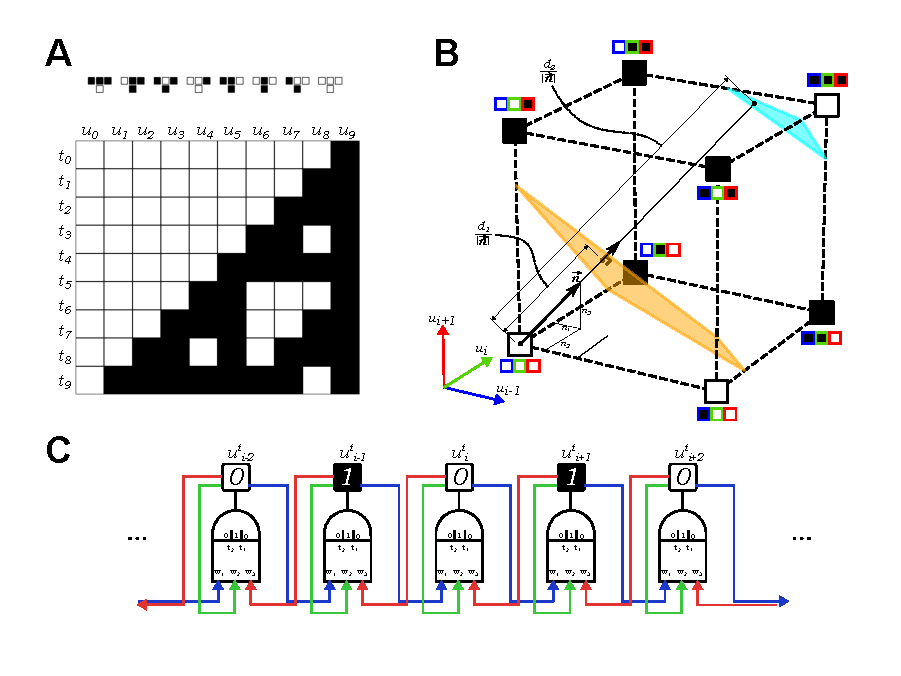
\includegraphics[width=\textwidth]{images/SVGs/Cube.pdf}
    \caption{A. The transition rule and time evolution of the Rule 110 cellular automata. B. Cube representation Rule 110 with separating planes defined by normal vector $\overrightarrow{n}$ and offset constants $d_1$ and $d_2$. The red, green and blue colouring corresponds to left neighbour, middle, and right neighbour cells of the neighbourhood respectively. C. Bi-threshold gate representation of an ECA architecture.}
    \label{fig:cube}
\end{figure}

% \subsection*{Bi-threshold Gates}

The result of this formulation of 3-input Boolean functions as linearly separable regions in a cube is the observation that most 3-input Boolean functions can be represented by a pair of parallel planes. This means we can translate a complicated Boolean algebraic expression composed of several AND, OR, XNOR, etc., gates into a single bi-threshold perceptron gate.

The bi-threshold perceptron for this ECA context can be formally represented as:


\begin{equation}
    f(N) = \begin{cases} 
0 & \text{if } \sum_{i=-1}^{1} w_i \cdot N_i > T_1 \\
1 & \text{if } T_2 \leq \sum_{i=-1}^{1} w_i \cdot N_i \leq T_1 \\
0 & \text{if } \sum_{i=-1}^{1} w_i \cdot N_i < T_2
\end{cases}
\end{equation}



\subsection*{Concept Mechanism}

In light of the mathematical formalism presented, we introduce a conceptual mechanical metamaterial designed to embody the logic and behavior of Elementary Cellular Automata (ECAs). This metamaterial is constructed from an array of interconnected unit cells, each serving as a mechanical analog to the bi-threshold pergeptron gate.

The core of each unit cell is a tristable element, functioning as the decision-making component. The tristable element has three stable states, akin to the three regions separated by the two parallel planes in the cube of our geometric representation. This element is responsible for holding the output state of the cell, dictated by the weighted sum of its inputs. 

Each unit cell is interconnected via coupling springs, which transmit mechanical signals between adjacent cells. The stiffness values of the coupling springs \(k_i\) act as the weights \( w_i \) in the bi-threshold perceptron equation. These values determine the force interactions and state transitions between adjacent unit cells. The tristable elements have multiple stable states, analogous to the regions separated by planes in the cube of our geometric ECA representation.

An input clock signal introduces a temporal dimension to the mechanical system, enabling dynamic state evolution similar to time-stepping in ECAs. This clock signal sets the computational cycle and synchronizes the unit cells.

Thus, the mechanical properties of the springs and tristable elements correspond directly to the mathematical constructs of the bi-threshold perceptron, providing a means to implement ECA rules in a mechanical system. The specific embodiment of this concept is detailed in the following section.

\subsection*{Unit cell design}
The unit cell is designed to be planar and monolithic for scalability, operate under a single shared clock signal for synchronization, transmit forces between adjacent cells, hold state in the absence of input, and transition states according to neighboring conditions. \autoref*{fig:Mechanism}A depicts the unit cell and its key components: the tristable element in teal, the bistable element in purple, the signal transmission element in orange, and the input bifurcation element in dark blue. Coupling springs, coloured in red, green, and blue, link the tristable element out-of-plane to the bifurcation elements of adjacent unit cells. The configuration of each unit cell is fully defined by two displacements: \(d^t\) in the \(\hat{e}_1\) direction for the tristable element and \(d^b\) in the \(\hat{e}_1\) direction for the bifurcation element ldue to the parallel links constraining rotational degrees of freedom. The input bifurcation element is so named because under actuation by an input clock signal \(\epsilon\), its shuttle block will displace a distance \(\delta\) in one of two directions, pushing or pulling on the coupling springs according to the state of the unit cell, "on" or "off" respectively. In order for the the bifurcation element to bifurcate only due to the configuration of the bistable element and not the tristable element, the operation of the unit cell requires the coupling springs to be \emph{tension-only} (\autoref*{fig:Mechanism}B). The details of this feature is elaborated in the next section. 

The bistable element acts as a mechanical binary memory element for the unit cell, while the tristable element's two snapthrough force thresholds act as decision boundaries corresponding to the thresholds of the threshold gate, or the separating planes of the boolean function. The signal transmission and bifurcation elements facilitate the temporal clocking and informational interconnection of the unit cells. 

A simplified pseudo-rigid body model of the unit cell is depicted in Figure \autoref*{fig:Mechanism}B. In this model, the contributions of numerous short-length flexure joints are aggregated into four torsional springs with angular stiffnesses \((k_\alpha, k_\beta, k_\gamma, k_\theta)\). These springs are subject to characteristic angular displacements \((\alpha, \beta, \gamma, \theta)\), which represent the angles of the tristable, bistable, signal transmission, and bifurcation links, respectively. The angles \(\alpha\), \(\beta\), and \(\gamma\) are part of a single-degree-of-freedom kinematic chain, while \(\theta\) and the input displacement \(\epsilon\) form another single-degree-of-freedom kinematic chain.
The bistable element is simplified using symmetry and modeled as a single-link slider with torsional stiffness \( k_\beta \) and a reaction/support stiffness \( k_r \). The transmission element is represented as a single link connecting the bistable element's shuttle block to a horizontal slider block. This link has a torsional stiffness \( k_\gamma \) and is guided by flexures with a support stiffness \( k_g \).
The signal transmission block is connected to the bifurcation element via a spring with stiffness \( k_s \). This spring is attached at a point located a distance \( h \) from the anchor pivot of the bifurcation element.
\todo{add h to figure}

\autoref*{fig:Mechanism}C shows the effect of the position of the tristable element on the behaviour of the bifurcation element under actuation. For each possible starting state configuration, the bifurcation element buckles accordingly. 


\begin{figure}[H]
    \centering
    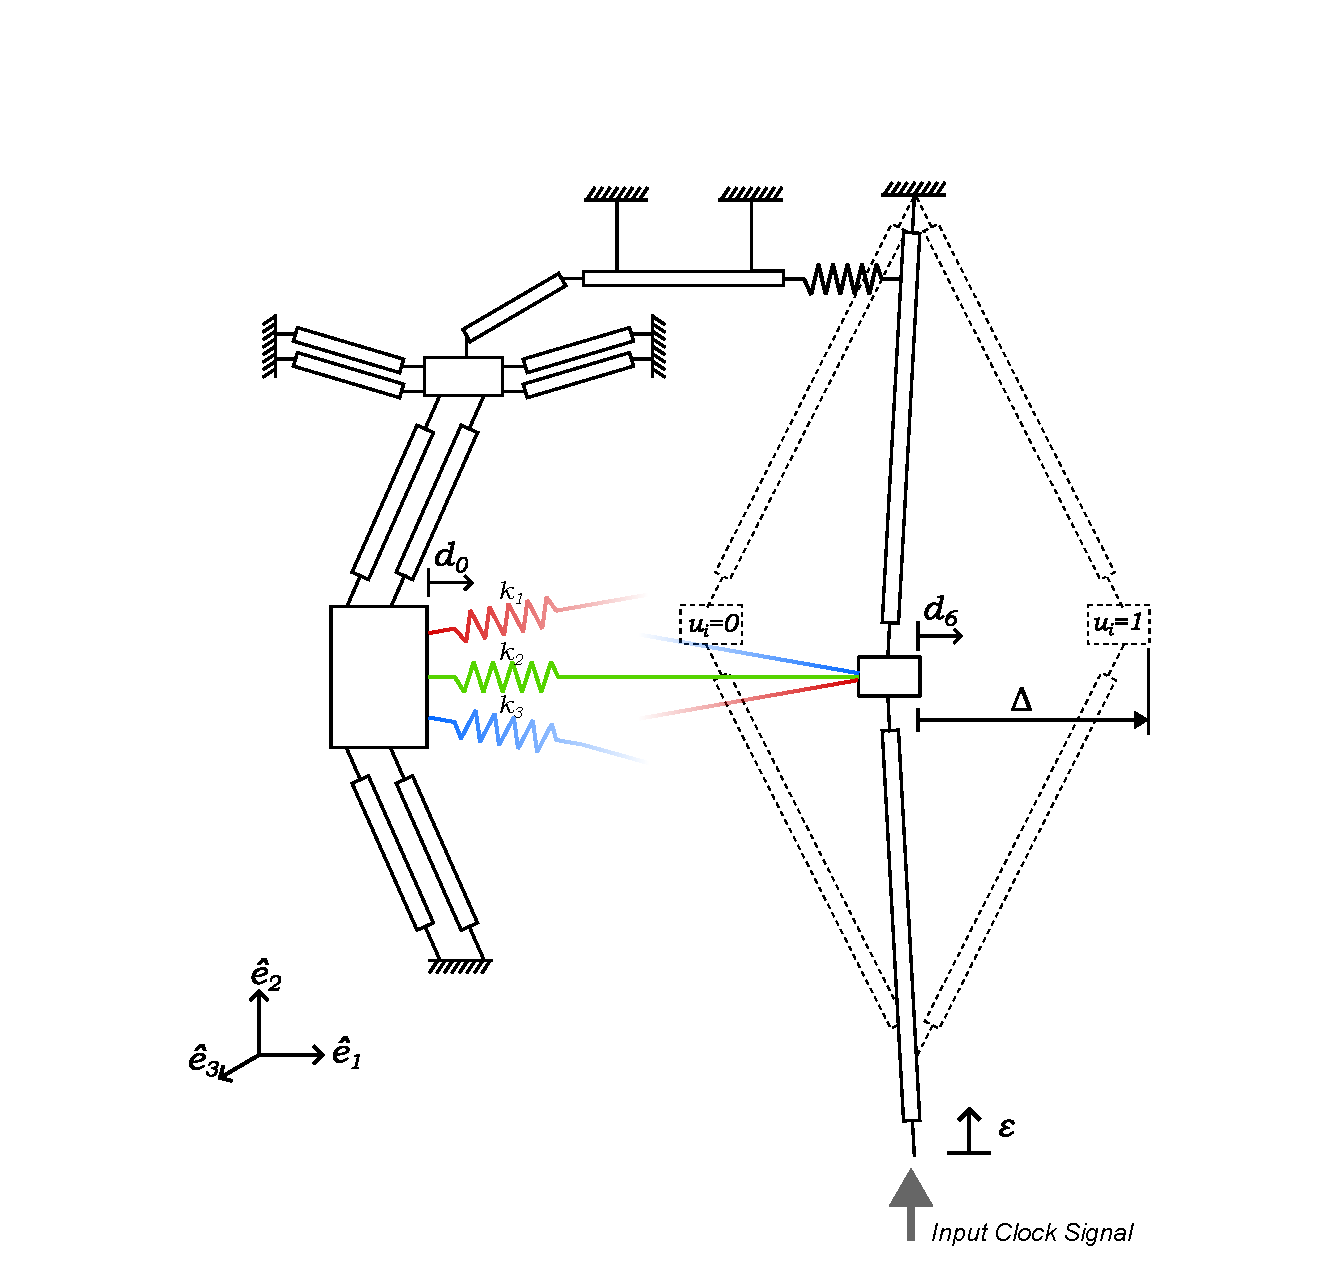
\includegraphics[width=\textwidth]{images/SVGs/PRBM.pdf}
    \caption{A. Compliant embodiment of unit cell design. B. Pseudo-rigid body model of unit cell. C. Bifurcation element displacement under actuation for each possible starting state configuration.}
    \label{fig:Mechanism}
\end{figure}



\subsection*{Working Principle/Kinetics}

\autoref*{fig:Equilibria and Tension-only spring}A shows the theoretical force-displacement behaviour of the tristable element, graphing the reaction force on the tristable shuttle as a function of its horizontal displacement \(d^t\). The three stable equilibria and corresponding configuration of the mechanism are shown. 
The specific behaviour is a function of all the joint stiffnesses and the chosen geometric dimensions and proportions of the mechanism. These design parameters must be precisely calculated and calibrated to achieve the precise desired behaviour, as variation can lead to mono-stable, bi-stable, or quad-stable behaviour. The specific derivation of the force-displacement response is detailed in Appendix \ref*{sec:Compliant Mechanism Design}.

\todo{Create appendix for this derivation}

The theoretical force-displacement behavior of the coupling tension-only springs is depicted in \autoref*{fig:Equilibria and Tension-only spring}B. Specifically, the spring behaves as a linear element with stiffness \( k_i \) when its elongation is positive. For negative elongation, the spring is slack, resulting in zero force. The stiffness \( k_i \) serves as a design parameter for selecting the specific ECA rule to be implemented.

\autoref*{fig:Equilibria and Tension-only spring}C illustrates a free-body diagram detailing the forces acting upon the tristable shuttle element. Here, \( F_r \) represents the total reaction force exerted by the tristable mechanism on the shuttle, while \( F_s \) denotes the cumulative force from all non-slack coupling springs. Equilibrium is achieved when the reaction and spring forces balance: \( F_r(d^t) = F_s(d^t, d^b) \). 

\begin{figure}[h]
    \centering
    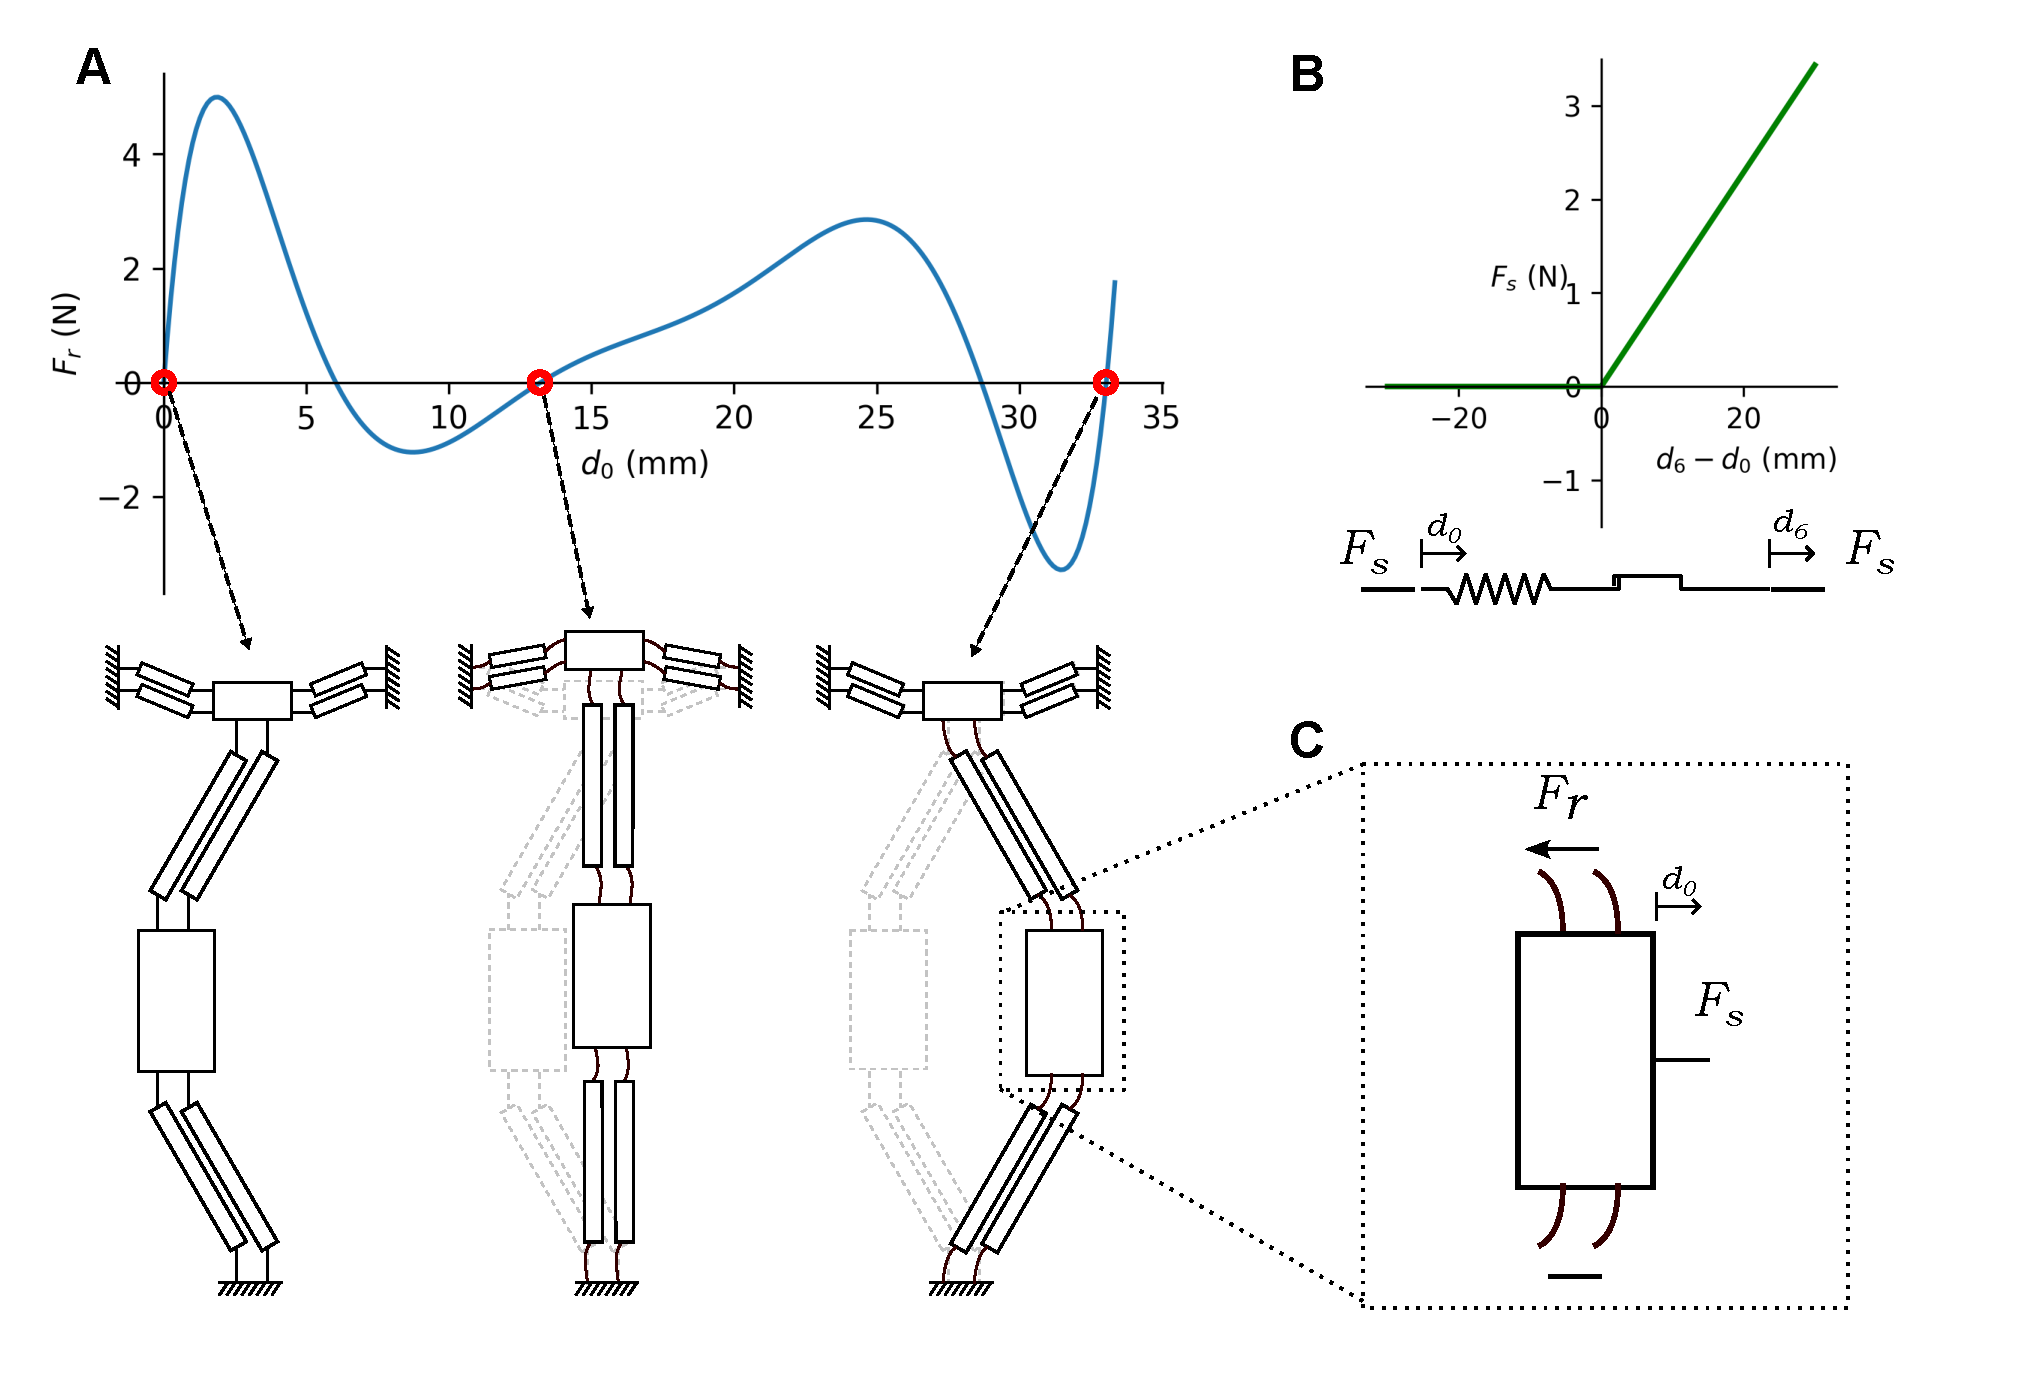
\includegraphics[width=\textwidth]{images/SVGs/Equilibria1.pdf}
    \caption{A. Force-displacement response of thethree stable equilibria and corresponding configurations of the state element. B. Force-displacement response of the tension only spring }
    \label{fig:Equilibria and Tension-only spring}

\end{figure}
    \todo{generate pdf of this figure and edit axis labels for dt etc}



In \autoref*{fig:Equilibria under actuation}, the force-displacement behavior of the unit cell is depicted under varying conditions of coupling spring activations. When the bifurcation shuttle is fixed at a displacement \( \delta \), denoted as \( d^b = \delta \), the cumulative force from the activated coupling springs is plotted alongside the force-displacement curve of the tristable element, \( F_r(d^t) \).

Equilibrium points emerge where these two force-displacement curves intersect and are represented as red dots on the difference plot. The equilibrium points correspond to the configurations where the cumulative force \( F_s \) from the coupling springs is equal to the reaction force \( F_r \) of the tristable element: \( F_r(d^t) = F_s(d^t, d^b) \).

Now, let's address the "disappearance" of the equilibrium points. An equilibrium point "disappears" when the force-displacement line of the activated coupling springs no longer intersects with specific regions of the \( F_r \) curve—specifically, the regions around its local maxima. This occurs when the slope of the force-displacement curve for the activated springs, pivoting about the point \( d^b = \delta \), not only fails to intersect but actually surpasses these local maxima regions of \( F_r(d^t) \).

In this context, snapthrough events happen as follows: the tristable element transitions from its current equilibrium state to an adjacent one depending on whether \( F_r < F_s \) or \( F_r > F_s \). This transition is triggered when the equilibrium state corresponding to the current \( F_r \) and \( F_s \) values no longer exists. This mechanical action serves as the physical embodiment of the decision boundaries in the bi-threshold perceptron.


\begin{figure}[H]
    \centering
    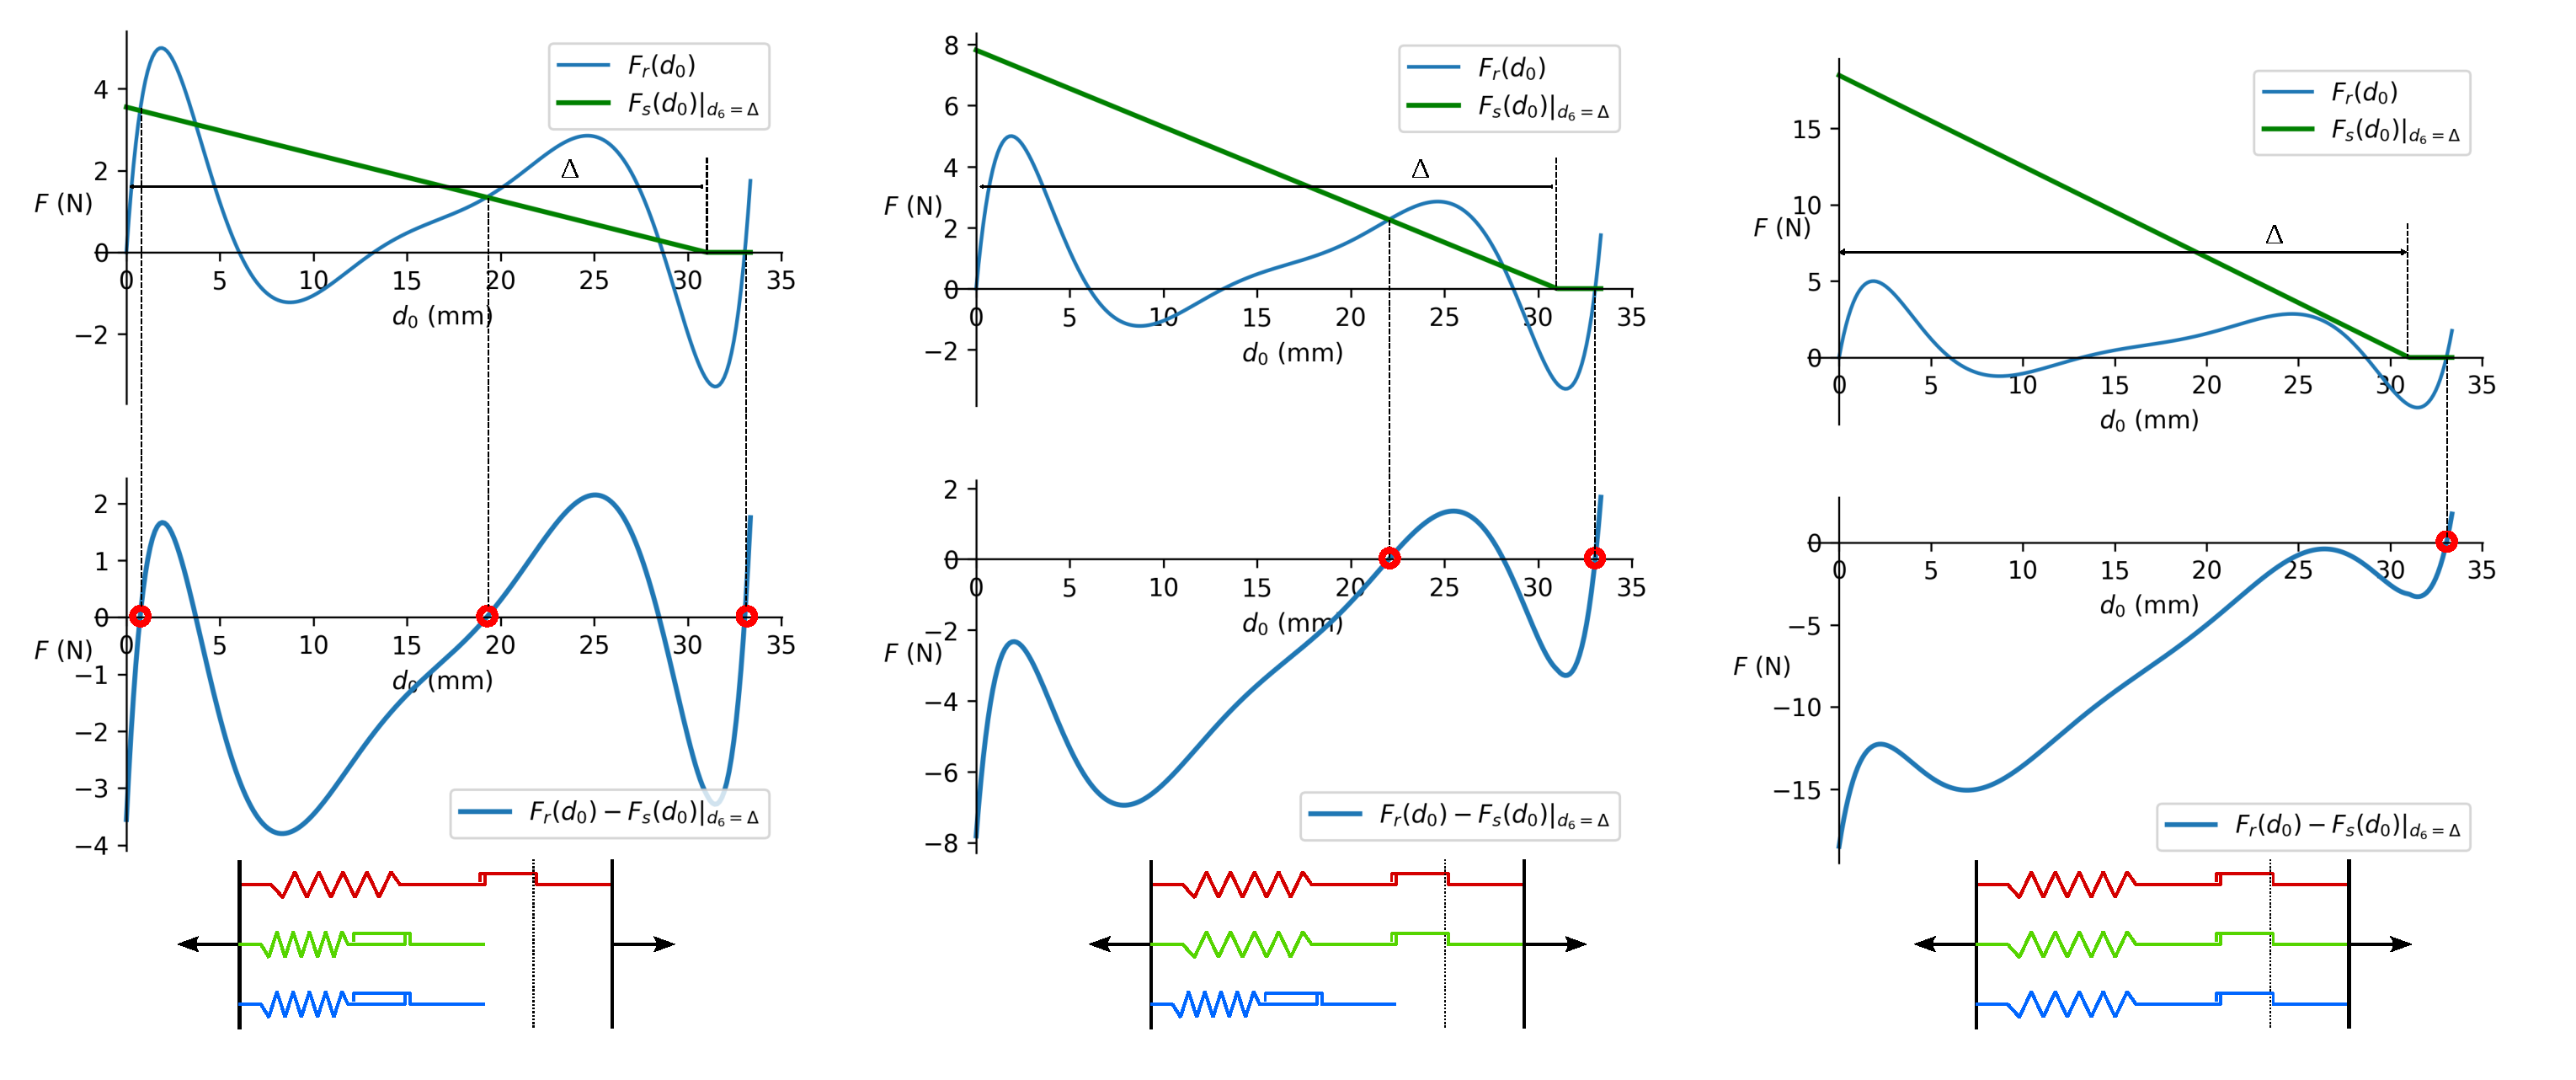
\includegraphics[width=\textwidth]{images/SVGs/Equilibria2.pdf}
    \caption{Force-displacement behavior with varying coupling spring activations. Equilibrium points, shown as red dots, emerge where the tristable element's reaction force \( F_r \) intersects with the cumulative spring force \( F_s \). Equilibria disappear when the spring force curve, anchored at \( d^b = \delta \), surpasses \( F_r \)'s local maxima, triggering a snapthrough event. This models the decision boundaries of a bi-threshold perceptron.}
    \label{fig:Equilibria under actuation}
\end{figure}

Recalling the mathematical formalism of ECA rules as bi-threshold perceptrons, we can now establish a direct correspondence between the mechanical and computational domains. In the bi-threshold perceptron model, the output state is determined by evaluating a weighted sum of inputs and comparing it against two threshold values \( T_1 \) and \( T_2 \):

\todo{add reference instead of repeating equation}

Here, \( w_i \) are the weights, and \( x_i \) are the input states from the neighborhood.

In the mechanical system, these weights \( w_i \) are analogous to the stiffness \( k_i \) of the coupling springs. The input states \( x_i \) correspond to the displacements \( d^b \) of the neighboring cells, a function of the states of their bistable elements. 
The thresholds \( T_1 \) and \( T_2 \) correspond to the critical effective stiffnesses of the cumulative active coupling springs at which the tristable element undergoes snap-through transitions. These critical effective stiffnesses are determined by the slopes of the lines that are tangent to the specific maxima regions on the \( F_r(d^t) \) force-displacement curve. These tangent lines are anchored at the point where \( d^b = \delta \) on the \( d^t \) axis.

\subsection*{Parametric determination of ECA rule}
\todo{move to methods}
Here we outline a parametric strategy for physically embodying a specific ECA rule, leveraging its geometric representation as parallel planes. The aim is to precisely calibrate the stiffness values \( k_i \) of the coupling springs and the maximum displacement \( \delta \) of the bifurcation element to manifest the desired ECA rule.

A pivotal insight is that modifying the bifurcation element's maximum displacement \( \delta \) alters the slopes of the lines tangent to the \( F_r(d^t) \) curve, as shown in \autoref*{fig:stiffness ratio}. These tangent lines are anchored at the point \( d^b = \delta \) on the \( d^t \) axis. This adjustment effectively varies the ratio between the bi-threshold perceptron's \( T_1 \) and \( T_2 \) values. Therefore, by selecting a specific \( \delta \), we can control the orientation of the separating planes, aligning them with the desired ECA rule. 

Subsequently, we can determine the coupling spring stiffnesses \( k_i \), which correspond to the slopes, which in turn correspond to the separating plane orientations, thereby completing the physical embodiment of the selected ECA rule.

However, the curve describing the critical stiffness ratio \( \frac{k_2}{k_1} \) as a function of \(\delta\) depends on the specific force displacement curve of the tristable element. 


\begin{figure}[H]
    \centering
    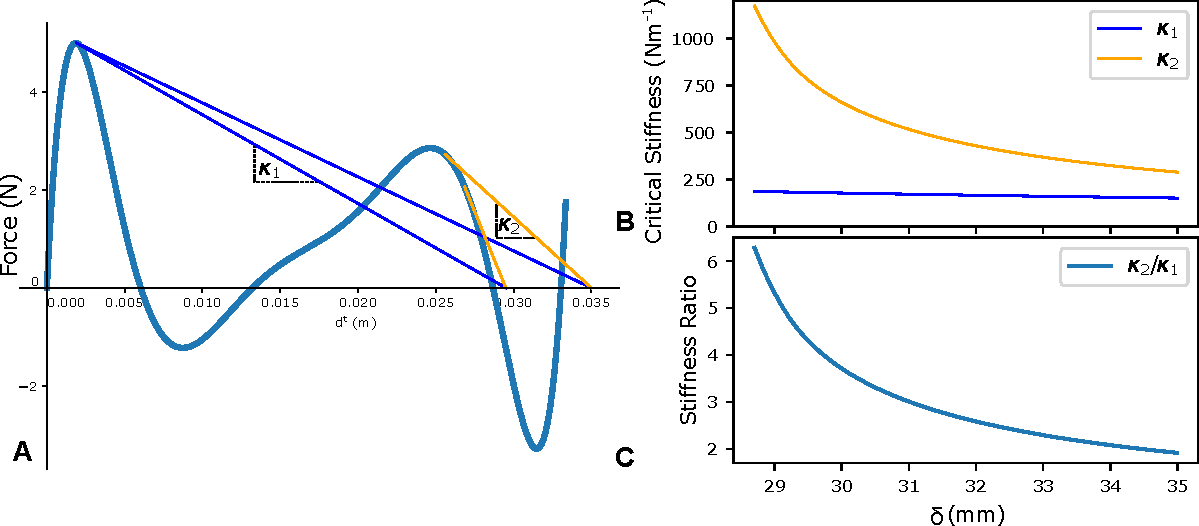
\includegraphics[width=\textwidth]{images/SVGs/stiffness_ratio.pdf}
    \caption{A. Force-displacement curve of the tristable with two different bifurcation element displacements \(\delta_1\), \(\delta_2\) showing the change in the slope of the tangent lines at the local maxima. B. Curves showing the critical stiffnesses \(k_1\) and \(k_2\) as a function of the bifurcation element displacement \(\delta\). C. Curve showing the critical stiffness ratio \(\frac{k_2}{k_1}\) as a function of the bifurcation element displacement \(\delta\)}
    \label{fig:stiffness ratio}
\end{figure}


\subsection*{Implementation of Rule 110}

To demonstrate the efficacy of this parametric design strategy, we implement Rule 110 in a physical prototype. The design process is as follows:

\begin{description}
    \item[Define Rule Characteristics] Each Elementary Cellular Automata (ECA) rule can be geometrically characterized by a normal vector \( \mathbf{n} = [n_1, n_2, n_3] \) and threshold values \( T_1 \) and \( T_2 \). For example, for Rule 110, \( \mathbf{n} = [1, 2, 2] \) and \( T_1 = 1.5, T_2 = 4.5 \).
    
    \item[Compute Critical Stiffness Ratio] The ratio of the threshold values, \( \frac{T_2}{T_1} \), serves as a critical parameter in the design. For Rule 110, \( \frac{T_2}{T_1} = 3 \).
    
    \item[Determine Bifurcation Displacement] The bifurcation displacement \( \delta \) corresponding to the critical stiffness ratio is determined by consulting \autoref*{fig:stiffness ratio}C. In the case of Rule 110, \( \delta \approx 31 \, \text{mm} \).
    
    \item[Calculate Critical Stiffnesses] The critical effective stiffnesses \( \kappa_1 \) and \( \kappa_2 \) are obtained from \autoref*{fig:stiffness ratio}B, based on the selected bifurcation displacement \( \delta \).
    
    \item[Compute Coupling Spring Stiffness] The stiffness \( k_i \) of each coupling spring is then derived using:
    \[
    k_i = \frac{n_i \times \kappa_1}{T_1}
    \]
\end{description}
 The bifurcation displacement is bounded below by the \(2L_a\cos(\alpha_0)\), in order for the input to fully actuate the tristable element. It is bounded above by the stress limits of the flexures on the bifurcation element. 

The final mechanical parameters for a given ECA rule, such as Rule 110, are summarized in \autoref*{tab:Parametric Design Values for Rule 110}.

\begin{table}[h]
\centering
\begin{tabular}{|c|c|c|c|c|c|c|}
    \hline
      & \( \kappa_1 \) & \( \kappa_2 \) & \( k_1 \) & \( k_2 \) & \( k_3 \) & \( \delta \) \\
    \hline
    Value & 171.81 & 515.39 & 114.54 & 229.08 & 229.08 & 31 \\
    \hline
    Units & \( \text{N/m} \) & \( \text{N/m} \) & \( \text{N/m} \) & \( \text{N/m} \) & \( \text{N/m} \) & \( \text{mm} \) \\
    \hline
    \end{tabular}
\caption{Summary of Parametric Design Values for Rule 110}
\label{tab:Parametric Design Values for Rule 110}
\end{table}

\autoref*{fig:Equilibria corresponding to Rule 110} demonstrates the one-to-one correspondence between the tristable element's equilibrium configurations and the cube representation of Rule 110. Each equilibrium state is directly tied to a specific combination of activated coupling springs. The relative effective stiffness of these springs, when compared to two critical stiffness thresholds, serves as the mapping M that locates each vertex relative to the separating planes in the cube representation.
\begin{figure}[H]
    \centering
    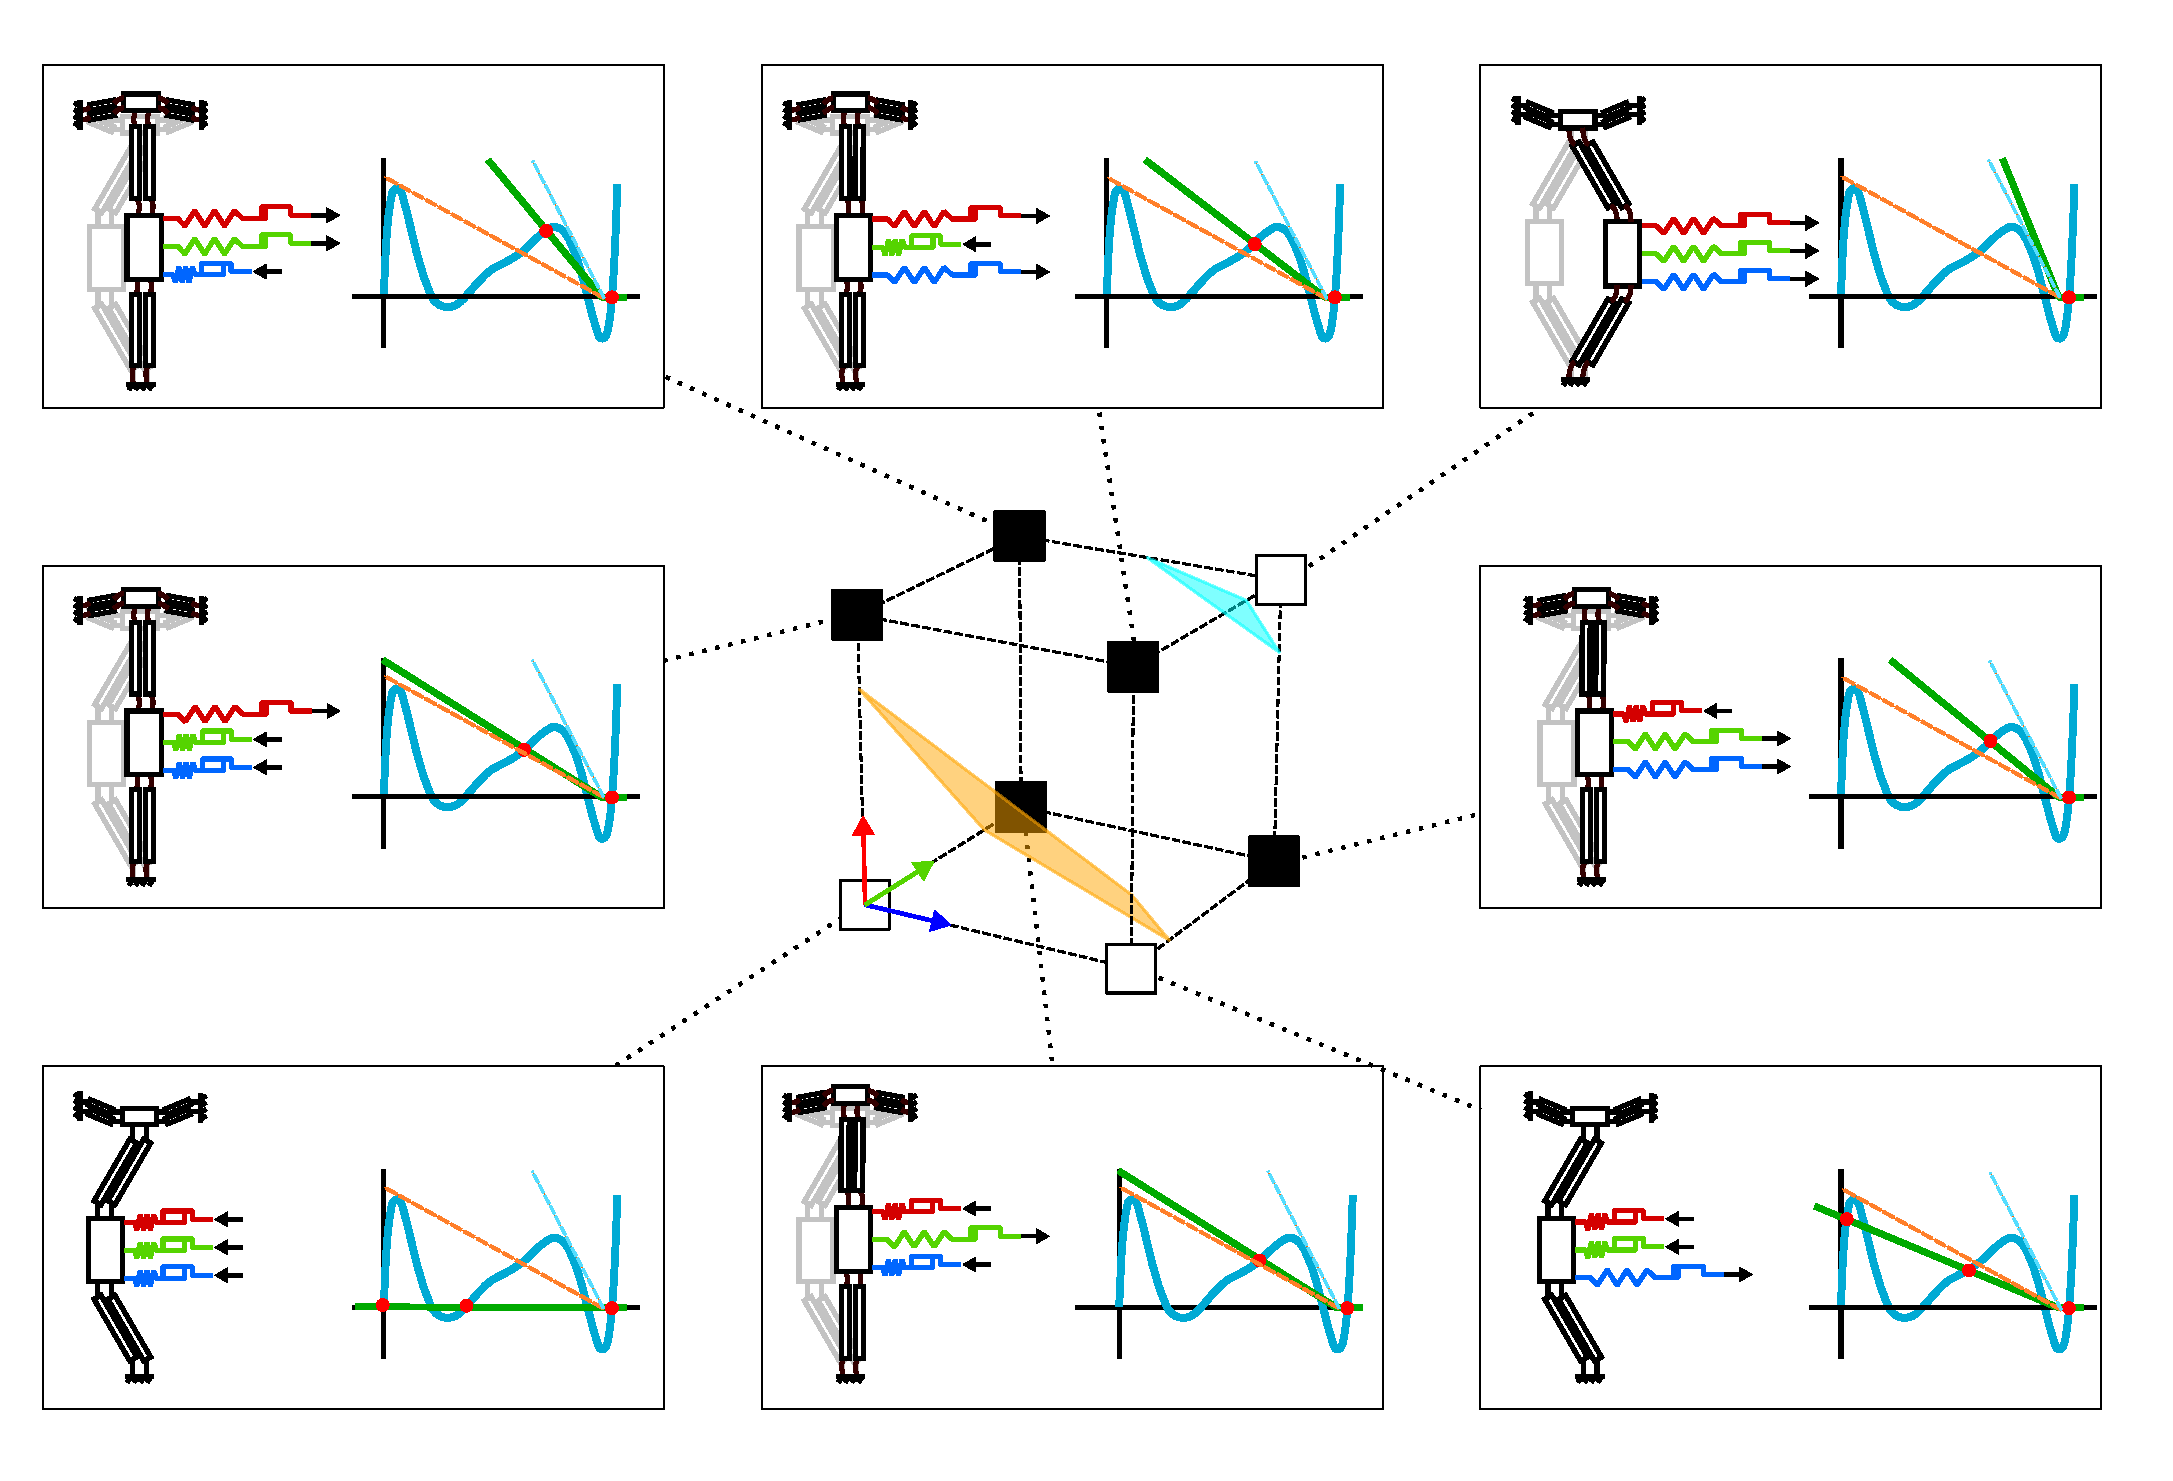
\includegraphics[width=\textwidth]{images/SVGs/Equilibria3.pdf}
    \caption{Equilibria of the tristable element corresponding to Rule 110. Each equilibrium state is directly tied to a specific combination of activated coupling springs. The relative effective stiffness of these springs, when compared to two critical stiffness thresholds, serves as the mapping M that locates each vertex relative to the separating planes in the cube representation.}
    \label{fig:Equilibria corresponding to Rule 110}
\end{figure}

\subsection*{Compliant Embodiment and FEA Modelling}

\subsubsection*{Tristable Mechanism}
As the previous section showed, the force displacement behaviour of the tristable mechanism is crucial to the performance of the unit cell as a logical element. Gou et al. \cite{Gou2021} developed a methodical design approach for monolithic compliant multistable structures. The approach employs a single bistable element with additional end effectors in series--which act effectively as frequency multipliers--to add extra stable points. In this paper, we use the same approach, selecting the architecture with a single additional end effector, which can result in a mechanism with 1, 2, 3, or 4 stable states, depending on the design parameters. First, a suitable bistable mechanism is selected and characterised. 
In our case, this is modelled as a single link-slider with initial angle \(\beta_0\), link length \(L_b\), bending stiffness \(k_\beta\) and compressive reaction-support stiffness \(k_r\). To convert the model to a compliant embodiment, these values are then converted to dimensional parameters of flexures and reinforced sections, based on the Young's modulus and flexural strength of the material to be used, as well as the constraints of the manufacturing method and the desired scale of the mechanism. 
Appropriate values for these parameters can be found in literature. We then fine-tuned the values with parameter sweeps in FEA and PRBM simulations. 

The end-effector compliant embodiment comprises of two pairs of parallel, lumped-compliance links and a moving end-effector block. The submechanism is parameterised by an initial link angle \(alpha_0\), link length \(L_a\) and combined flexural stiffness \(k_\alpha\). These are calculated to satisfy the following conditions: 
\begin{itemize}
    \item The bistable element is at its second equilibrium position when the end effector is in the central configuration, i.e. \(\alpha = 0^\circ\).
    \item The retaining force of the bistable element in its second equilibrium position is greater than the peak reaction force generated by the end effector flexures in the central configuration.
    \item The snapthrough force of the bistable element is greater than the peak reaction force generated by the end effector flexures in the right-most configuration.
    \item The buckling load of the end effector flexures is greater than the peak reaction force of the bistable element.
\end{itemize} 

These conditions impose upper and lower bounds on the design parameters, which can be used to determine the appropriate values for the end effector parameters. The full design process can be found in the cited paper\cite{Gou2021}. 
\todo{These conditions are not very clear. Maybe add a figure? Or can we just say that we used the same design process as the paper?}


\subsubsection*{Coupling Springs}
The coupling springs are modelled as linear springs with stiffness \(k_i\). The stiffness values are calculated using the parametric design strategy outlined in the previous section. The springs are designed to be tension-only, i.e. they are slack when the bifurcation mechanism buckles to the left, signalling "off". This can be achieved in embodiment by several methods, such as a contact-based latch system \cite{Gao2019}, or by using a buckling flexure with a very small buckling load. The latter approach is assumed in this paper, as it is the simplest to implement. The buckling force of a leaf flexure can be calculated by \(F_b = \frac{\pi^2EI}{L_b^2}\), where \(E\) is the Young's modulus of the material, \(I\) is the second moment of area of the flexure cross-section, and \(L_b\) is the length of the flexure. The buckling force can be arbitrarily reduced by increasing the length of the flexure and keeping \(I\) sufficiently small. 

The coupling springs were designed as serpentine springs with a single buckling flexure. The spring is defined by the following parameters: spring leg length \(L_s\), number of legs \(N\), and the moment of inertia of the spring leg cross section \(I\)
The spring must be designed such that at maximum extension \(\Delta\), the stress does not exceed the yield stress of the material \(\sigma_{\text{max}}\), which can be calculated by\( \sigma_{\text{max}} = \frac{k_i\Delta L t}{4I} \). Rearranging this gives an upper bound on the length of each leg: \( L_{\text{max}} = \frac{\sigma_{\text{max}}4I}{k_i \Delta} \). The total stiffness of the spring is given by \( k_i = \frac{12E I}{L^3 N} \), as the legs act as springs in series. This formula gives a lower bound on \(N\) to satisfy the range of motion constraint using \( N = \frac{12E I}{L_{\text{max}}^3 k_i} \). Together these allow the selection of a suitable spring design, that satisfies any form factor constraints.
\( L_s = \sqrt[3]{\frac{12E I}{N k_i}} \)
The table below shows the calculated parameters for one possible embodiment of the tristable element and coupling springs to implement Rule 110:
\todo{placeholder values}


\begin{tabular}{|c|c|c|c|c|c|c|c|c|c|c|c|c|c|}
    \hline
    Parameter & \( w \) & \( t1 \) & \( t2 \) & \( t3 \) & \( BL1 \) & \( BL2 \) & \( h \) & \( sl \) & \( st \) & \( Lr1 \) & \( L1 \) & \( \beta_0 \) & \( \alpha_0 \) \\
    \hline
    Value & 5 & 0.4 & 2.5 & 2.5 & 4 & 24 & 5 & 6 & 2 & 35 & 6 & 8 & 22 \\
    \hline
    Units (mm or \( ^\circ \)) & mm & mm & mm & mm & mm & mm & mm & mm & mm & mm & mm & \( ^\circ \) & \( ^\circ \) \\
    \hline
    \end{tabular}

\subsubsection*{FEA Validation of Tristable Element \& Coupling Spring}

Ansys APDL was used to validate the design of the tristable element and coupling springs determined by the PRB model. The sub-mechanisms were modelled using BEAM188 elements with linear elastic material to represent the flexures. \todo{What details are essential to include here?} The coupling springs stiffness was validated by applying a fixed extension to the spring and measuring the reaction force. The tristable element was validated using a displacement boundary condition on the tristable shuttle, and measuring the reaction force, as the snapthrough behaviour prevents convergence when a force boundary condition is applied. The snapthrough and bi-threshold behaviour was validated by applying a displacement boundary condition to all combinations of coupling springs using arc-length loading method and determining the equilibrium states. The bifurcation and signal transmission components were also validated to demonstrate the state-dependent buckling behaviour of the input mechanism. The results of the FEA validation are shown in \autoref*{fig:FEA}.

\begin{figure}
    \centering
    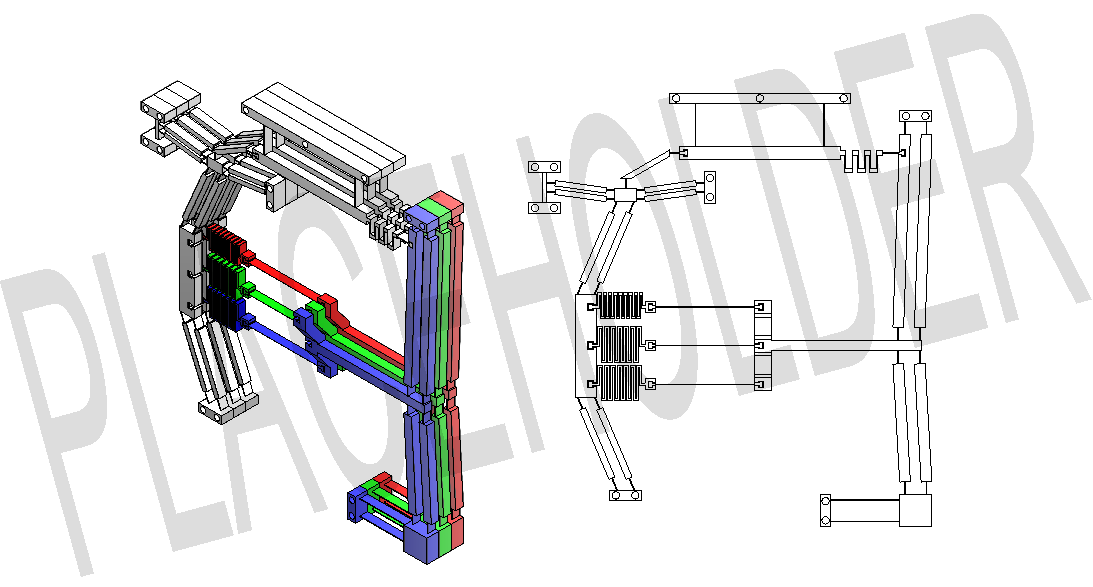
\includegraphics[width=\textwidth]{images/SVGs/v5Assembly.pdf}
    \caption{CAD representation of periodic arrangement of the prototype. The coloured bifurcation elements of the neighbourhood all connect to the central cell. The coupling springs of the neighbours are not shown for clarity. }
    \label{fig:Prototype}
\end{figure}
\subsection*{Pseudo-Rigid Body Modelling}

The culmination and main result of the theoretical framework and concept mechanism developed thus far is a pseudo-rigid body model simulation of the unit cell and complete system, implemented in a custom Python script. The simulation implements the kinematics and kinetics of the simplified unit cell in \autoref*{fig:Mechanism}B, and models the nonlinear interaction between cells, and the simultanoeous actuation of the bifurcation mechanisms. 
\todo{explain basic procedure}
The simulation's objectives are twofold:
\begin{enumerate}
    \item To produce the force-displacement graphs that enable the parametric design strategy for implementing a specific ECA rule.
    \item To provide a computational testing ground for the system's time evolution, thereby serving as a preliminary validation of the parametric design strategy for embodying a specific ECA rule.
\end{enumerate}


The simulation considers each cell having two degrees of freedom corresponding to the displacements of the tristable shuttle \( d^t \) and the bifurcation shuttle \( d^b \), modelled as link angles \(\alpha\) and \(\theta\) respectively. Intermediate angular and linear displacements of the spring elements are calculated using the forward kinematics of the PRBM. The total energy of each unit cell and the coupling springs, as well as the reaction torques on the degrees of freedon are calculated using the pseudo-rigid body model. The energy of each spring is calculated using the linear spring force-displacement relationship. A triangular wave function represents the clock signal 
\(varepsilon\), with amplitude derived from the bifurcation element's maximum displacement \(\delta\) as per the chosen ECA rule. The simulation advances in 1000 timesteps per actuation cycle. Equilibrium states are resolved at each timestep by minimising the system's total energy. This is achieved using Sequential Least Squares Programming with derivative information, with each new timestep initialized to the previous state's equilibrium.


The comprehensive codebase for the simulation can be found in Appendix \ref*{sec:Python Script for Pseudo-Rigid Body Simulation}.

\section{Results}


\subsection*{FEA Validation of Tristable Element \& Coupling Spring}

\autoref*{fig:FEA} shows the snapthrough behaviour of the tristable element under three different equivalent stiffness configurations in the Ansys APDL FEA model. 

\begin{figure}[H]
    \centering
    \includegraphics[width=\textwidth]{images/SVGs/FEAresults.pdf}
    \caption{A. Snapthrough behaviour of the tristable element under three different equivalent stiffness configurations in the Ansys APDL FEA model. B. Validation of the bifurcation state dependent behaviour. C. Validation of the derived force displacement behaviour of the tristable element.}
    \label{fig:FEA}
\end{figure}


\subsection*{Psuedo-Rigid Body Model Simulation}

\autoref*{fig:Simulation}A shows a representation of the initial states and final of a a 10-unit cell system at \(t_0\) and \(t_{10}\). The system is initialized with a single 'on' cell at the rightmost edge of the domain
\autoref*{fig:Simulation}B portrays a time series simulation of the system. The states of the cells evolve in accordance with transition Rule 110. The clock signal \( \epsilon \) is represented in orange. Each unit cell's bifurcation element orientation is indicative of its state—positive angle \( \theta \) equates to 'off', while negative \( \theta \) signifies 'on', as a negative angle implies pulling on the tension only spring. 

\autoref*{fig:Simulation}C shows the total potential energy \(E\) of the system over time, and the reaction force \(F\) calculated as the derivative of the potential energy with respect to the clock signal displacement \(\varepsilon\). The energy graph is discontinuous due to the snapthrough events of the tristable elements. The magnitudes of both the energy and reaction force are proportional to the number of unit cells in the system, as well as a funciton of the number of "on" cells, as this determines the number of active coupling springs. The reaction force is also proportional to the stiffness of the coupling springs, which is a function of the ECA rule being implemented. In timestep 8, when the maximum number of cells are "on", the reaction force is at its maximum value, and the peak energy also occurs due to the energy stored in the bistable elements. 





\begin{figure}[H]
    \centering
    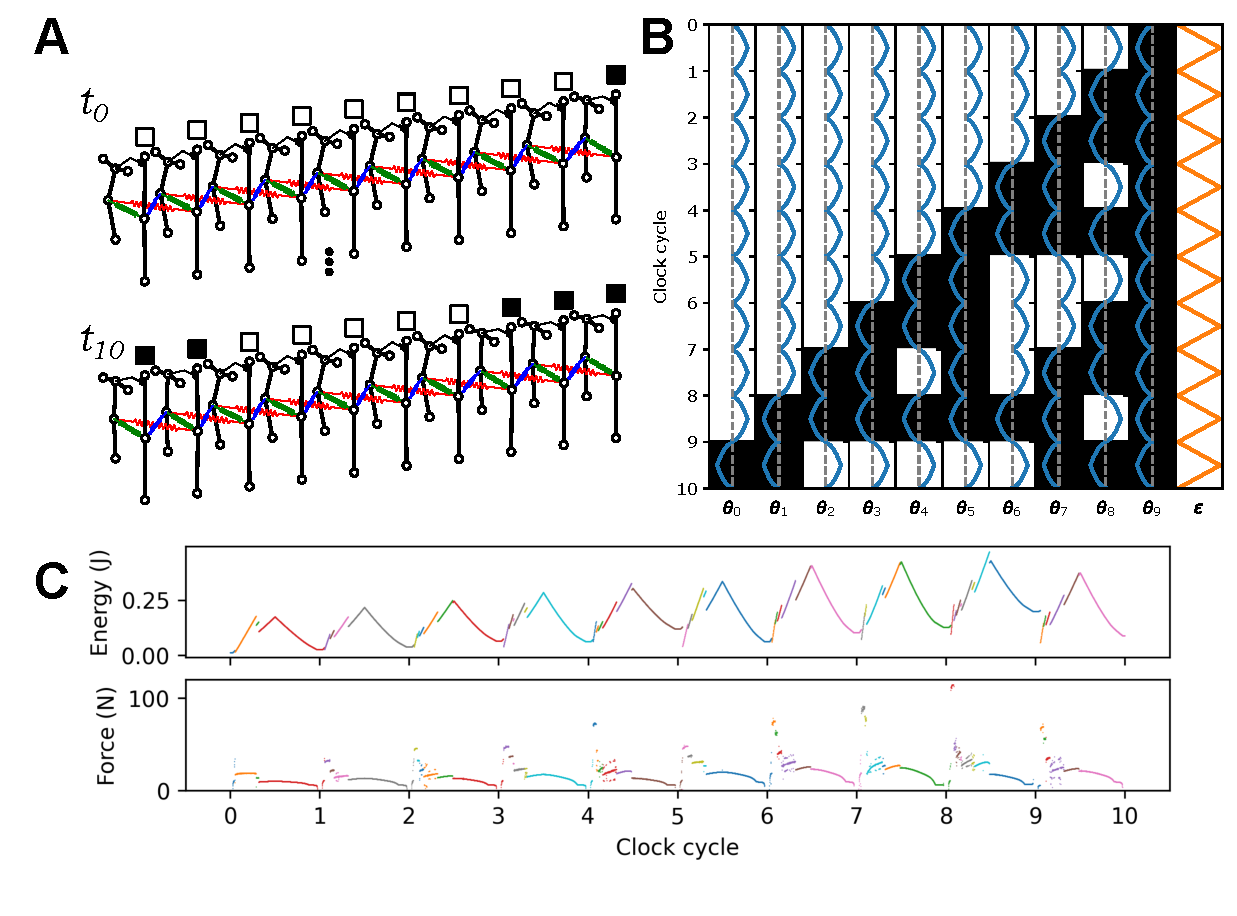
\includegraphics[width=\textwidth]{images/SVGs/Simulation.pdf}
    \caption{A. Rendering of psuedo-rigid body model at \(t_0\) and \(t_{10}\) showing arrangement of unit cells and interconnecting springs. B.Time series simulation of the system with 10 unit cells. Positive angle \(\theta\) correspons to the "off" state of the unit cell, while negative angle \(\theta\) corresponds to the "on" state. The clock signal \(\epsilon\) is shown in orange. The system evolves from a single "on" cell at the right edge of the domain according to Rule 110. C. The total energy of the system and reaction force felt by the input displacement boundary condition \(\varepsilon\).}
    \label{fig:Simulation}
\end{figure}




\section{Discussion}

\begin{itemize}
    \item Equivalence classes of ECA rules that can be implemented
    \item Constraints of design approach
    \item Manufacturability difficulties
    \item Scalability
    \item Limitations of pseudo-rigid body model
    \item Limitations of ECAs as a computing architecture
    \item Potential applications

\end{itemize}
While this paper has shown the calculation procedure for the implementation of Rule 100, the design strategy presented here can be applied to any ECA rule that is either linearly or bi-linearly separable, with some additional constraints. The normal vector of the separating planes must must have only non-negative components as the weights represent the physical property of spring stiffness, which cannot be negative. Additionally, with the current mechanism design, the rule must also satisfy the condition of null quiescence, it must output 'off' for an entirely 'off' neighbourhood i.e. \(f(0,0,0) =0\). \autoref*{fig:hypercubes} shows the hypercubes of 10 bi-threshold ECA rules that satisfy these conditions. Not shown are rules with only a single threshold, as they are trivially linearly separable, and the rules which are equivalent to those shown under permutation of the inputs. The complete set of possible rules is tabulated in Appendix %\ref*{sec:Complete Set of Bi-threshold ECA Rules}.

\begin{figure}[H]
    \centering
    \includegraphics[width=\textwidth]{images/SVGs/hypercubes.pdf}
    \caption{Cube representation of representative rules from the equivalence classes of bi-threshold ECA rules that can be implemented using the proposed design strategy. This is not exhaustive of all rules that can be implemented.}
    \label{fig:hypercubes}
\end{figure}






% \section{Conclusion}
